\documentclass[a4paper]{article}

% Pacotes para o português.
\usepackage[brazilian]{babel}
\usepackage[utf8]{inputenc}
\usepackage[T1]{fontenc}

\usepackage{datetime}
\usepackage{graphicx}

% Usado nos pedaços de código.
\usepackage{listings}
\lstset{language=C,
	basicstyle=\small\sffamily,
	numbers=left,
	numberstyle=\tiny,
	frame=tb,
	columns=fullflexible,
	showstringspaces=false,
	captionpos=b}
\renewcommand\lstlistingname{Código}

% Remove as identações.
\setlength{\parindent}{0in}

\newcommand{\HRule}{\rule{\linewidth}{0.5mm}}

\begin{document}

\begin{titlepage}
\begin{center}	

% Topo 1.
\textsc{\Large UNIVERSIDADE DE SÃO PAULO\\
	INSTITUTO DE CIÊNCIAS MATEMÁTICAS E DE COMPUTAÇÃO}\\[0.7cm]

% Topo 2.
\textsc{\Large SSC0143}\\[0.2cm]
\textsc{\Large Programação Concorrente - Turma B}\\[0.5cm]

% Título.
\HRule \\[0.4cm]
{ \huge \bfseries Algoritmos para realizar o cálculo aproximado do número \begin{math}\pi\end{math}}\\[0.4cm]
\HRule \\[1.5cm]

% Grupo e professor.
\begin{minipage}{0.4\textwidth}
\begin{flushleft} \large
\emph{Grupo:}\\
Bruno Junqueira Adami\\
Lucas Junqueira Adami\\
Lucas Lobosque
\end{flushleft}
\end{minipage}
\begin{minipage}{0.4\textwidth}
\begin{flushright} \large
\emph{Professor Dr.:}\\
Julio Cezar Estrella
\end{flushright}
\end{minipage}

\vfill

% Rodapé.
{\large \today}
	
\end{center}
\end{titlepage}

\section{Introdução}
\subsection{Algoritmo de Gauss-Legendre}
O algoritmo de Gauss-Legendre, baseado no trabalho individual de Carl Friedrich Gauss 
e Adrien-Marie Legendre, é um algoritmo para calcular os dígitos de \begin{math}\pi\end{math}. Sua
característica principal é sua convergência rápida, de segunda ordem, onde 24 
iterações produzem 10 milhões de dígitos corretos de \begin{math}\pi\end{math}. Ele segue os seguintes 
passos:

\begin{displaymath}
	a_0 = 1
\end{displaymath}
\begin{displaymath}
	b_0 = 1 / \sqrt{2}
\end{displaymath}
\begin{displaymath}
	t_0 = 1 / 4
\end{displaymath}
\begin{displaymath}
	p_0 = 1
\end{displaymath}
\\
\begin{displaymath}
	a_{n+1} = \frac{a_n + b_n}{2}
\end{displaymath}
\begin{displaymath}
	b_{n+1} = \sqrt{a_{n}b_{n}}
\end{displaymath}
\begin{displaymath}
	t_{n+1} = t_n - p_{n}(a_n - a_{n+1})^2
\end{displaymath}
\begin{displaymath}
	p_{n+1} = 2p_n
\end{displaymath}

\subsection{Algoritmo de Borwein}
O algoritmo de Borwein, criado pelos matemáticos Jonathan e Peter Borwein, é 
usado para calcular o valor de \begin{math}\pi\end{math}, com a precisão aumentando a cada iteração.
Existem várias versões do algoritmo. A versão utilizada no trabalho quadruplica 
o número de dígitos corretos a cada iteração, gerando 10 milhões de dígitos em 
apenas 12 iterações. Ela segue os seguintes passos:

\begin{displaymath}
	a_0 = 6 - 4\sqrt{2}
\end{displaymath}
\begin{displaymath}
	y_0 = \sqrt{2} - 1
\end{displaymath}
\\
\begin{displaymath}
	y_{k+1} = \frac{1 - (1-y_k^4)^\frac{1}{4}}{1 + (1-y_k^4)^\frac{1}{4}}
\end{displaymath}
\begin{displaymath}
	a_{k+1} = a_k(1 + y_{k+1})^4 - 2^{2k+3}y_{k+1}(1 + y_{k+1} + y_{k+1}^2)
\end{displaymath}

\subsection{Algoritmo de Monte Carlo}
O algoritmo de Monte Carlo é um método estatístico para calcular funções complexas
de um modo aproximado. Este método tipicamente envolve a geração de observações de 
alguma distribuição de probabilidades e o uso da amostra obtida para aproximar a 
função de interesse. As aplicações mais comuns são em computação numérica para avaliar 
integrais. A ideia do método é escrever a integral que se deseja calcular como um valor 
esperado. Foi utilizado este método para calcular a área de 1/4 do círculo. A partir 
deste valor, é possível estimar o valor do \begin{math}\pi\end{math}. O número de iterações do algoritmo determina 
a precisão do cálculo, cada casa decimal a mais multiplica um fator de 10x na quantidade
de iterações necessárias para tal. Mesmo tendo várias casas decimais, isso
não implica que as casas estão corretas. Além disso, o raio pode ser um valor arbitrário. 
Foi utilizado como raio o maior número aleatório possível.

\begin{displaymath}
	Area = \frac{\pi R^2}{4}
\end{displaymath}
\begin{displaymath}
	\pi = 4\frac{Area}{R^2}
\end{displaymath}
\begin{displaymath}
	Area = \frac{{Pontos Dentro do Circulo}}{{Pontos Totais}}
\end{displaymath}
\begin{displaymath}
	\pi = 4\frac{{Pontos Dentro do Circulo}}{{Pontos Totais}}
\end{displaymath}

\begin{lstlisting}[caption=Algoritmo de Monte Carlo, float=h]
pontosDentro = 0
pontosTotais = 0
M = 1000000000 // 10^9: 9 casas no resultado

pontosTotais = M

fazer M iteracoes
	a = rand()
	b = rand()
	se sqrt(a*a + b*b) <= r
		++pontosDentro
		
retornar 4*pontosDentro/pontosTotais
\end{lstlisting}

\section{Soluções}
Para os algoritmos de Gauss-Legendre e Borwein, foi utilizada a biblioteca GNU MP, uma 
biblioteca open-source para as linguagens C e C++ que é capaz de criar números 
com infinitas casas decimais. Ela foi usada porque as variáveis do tipo double 
não alcançam essa precisão. Para o algoritmo do Monte Carlo, não foi utilizada 
nenhuma biblioteca de números grandes, pois iria ser necessário mais do que \begin{math}10^{19}\end{math} 
iterações para justificar o uso.

\subparagraph{Números aleatórios no algoritmo de Monte Carlo:}
No C é possível usar a função rand() da stdlib para gerar os números aleatórios. Porém, segundo
o padrão do C, a função não é thread-safe, ou seja, não há garantias quanto ao uso desta função
em várias threads. Investigando mais a fundo, a implementação da função rand() pela libc usa
locks de contexto, isto é, apenas uma thread por vez pode chamar a função rand(). Isso iria
aumentar drasticamente o tempo do algoritmo, funcionando como algo serial. Então, foi implementado 
um gerador congruente linear, usando parâmetros parecidos com o mesmo usado pelo gcc, de tal modo 
que o gerador seja uniforme.\\

\begin{lstlisting}[caption=Algoritmo do gerador congruente linear, float=h]
X(n+1) = (A*X(n)+C) % M
X(0) = time(NULL) // numero inicial (seed) de acordo com o tempo atual..
A = 1103515245
C = 12345
M = 2^31
\end{lstlisting}

O maior número aleatório gerado é \begin{math}2^{31} - 1\end{math} (cabe em um inteiro de 32 bits com sinal, int em C no gcc). 
Este valor foi usado para a conta logo abaixo caber num inteiro de 64 bits com sinal (long long em C no gcc), 
Para não precisar usar o módulo no gerador, os bits são apenas truncados nas contas, deixando mais 
rápido os cáculos, por isso o módulo é \begin{math}2^{31}\end{math}. Para verificar se o ponto está dentro do círculo não é preciso 
usar pontos flutuantes ou raiz quadrada, deixando os cálculos mais rápidos e precisos:

\begin{displaymath}
	R = \sqrt{a^2 + b^2}
\end{displaymath}
\begin{displaymath}
	R^2 = a a + b b
\end{displaymath}

\subsection{Método sequencial}
O algoritmo de Monte Carlo foi implementado seguindo os passos descritos anteriormente. 
O número que é impresso na tela é o \begin{math}\pi\end{math} tirando a vírgula (ex: 3,1415 = 31415). 
Nos algoritmos de  Gauss-Legendre e Borwein, que são iterativos, variáveis auxiliares
(com sufixo \_) foram utilizadas para guardar os resultados da iteração anterior. O
valor de \begin{math}\pi\end{math} é mostrado em cada iteração.

\subsection{Método paralelo}
No método paralelo, foi utilizada a biblioteca pthreads (POSIX Threads) para 
a criação das threads do programa. No algoritmo de Monte Carlo, foram criadas N threads. 
Cada thread é responsável por gerar M' pontos. Se multiplicarmos M' por N teremos 
o M utilizado no método sequencial, ou seja, cada thread gera um pouco dos M pontos aleatórios. 
No fim tudo é somado obtendo o número esperado. Observe que as threads são independentes, 
não precisando de mutex ou sincronizações. No algoritmo de Borwein, foram utilizadas duas threads, uma para 
calcular \begin{math}y_{k+1}\end{math} e outra para calcular \begin{math}a_{k+1}\end{math}.
No algoritmo de Gauss-Lagrange, foram criadas três threads, uma para calcular
\begin{math}a_{n+1}\end{math} e \begin{math}t_{n+1}\end{math}, outra para calcular \begin{math}b_{n+1}\end{math} e
a última para calcular \begin{math}p_{n+1}\end{math}.

\section{Resultados e conclusões}
Nos experimentos, o comando time do Linux, que conta o tempo de execução de um 
processo, foi utilizado. Além disso, os comandos de impressão dos dígitos de \begin{math}\pi\end{math} 
foram removidos para que apenas o tempo de processamento fosse computado. Para o
algoritmo de Monte Carlo, foram testados várias quantidades de threads, com a otimização
O3 e sem. Para os outros dois algoritmos, as otimizações O3, O2, O1 e sem otimização foram
utilizadas. Além disso, para os algoritmos que utilizaram a GNU MP, a precisão passada
à biblioteca foi 3.32 maior que 10 milhões, pois este número não é necessariamente a precisão final. 
Portanto, o número de iterações nesses casos foi um pouco maior. Esse valor foi calculado empiricamente.\\

\begin{figure}[float=h]
	\begin{center}
		\scalebox{0.5}{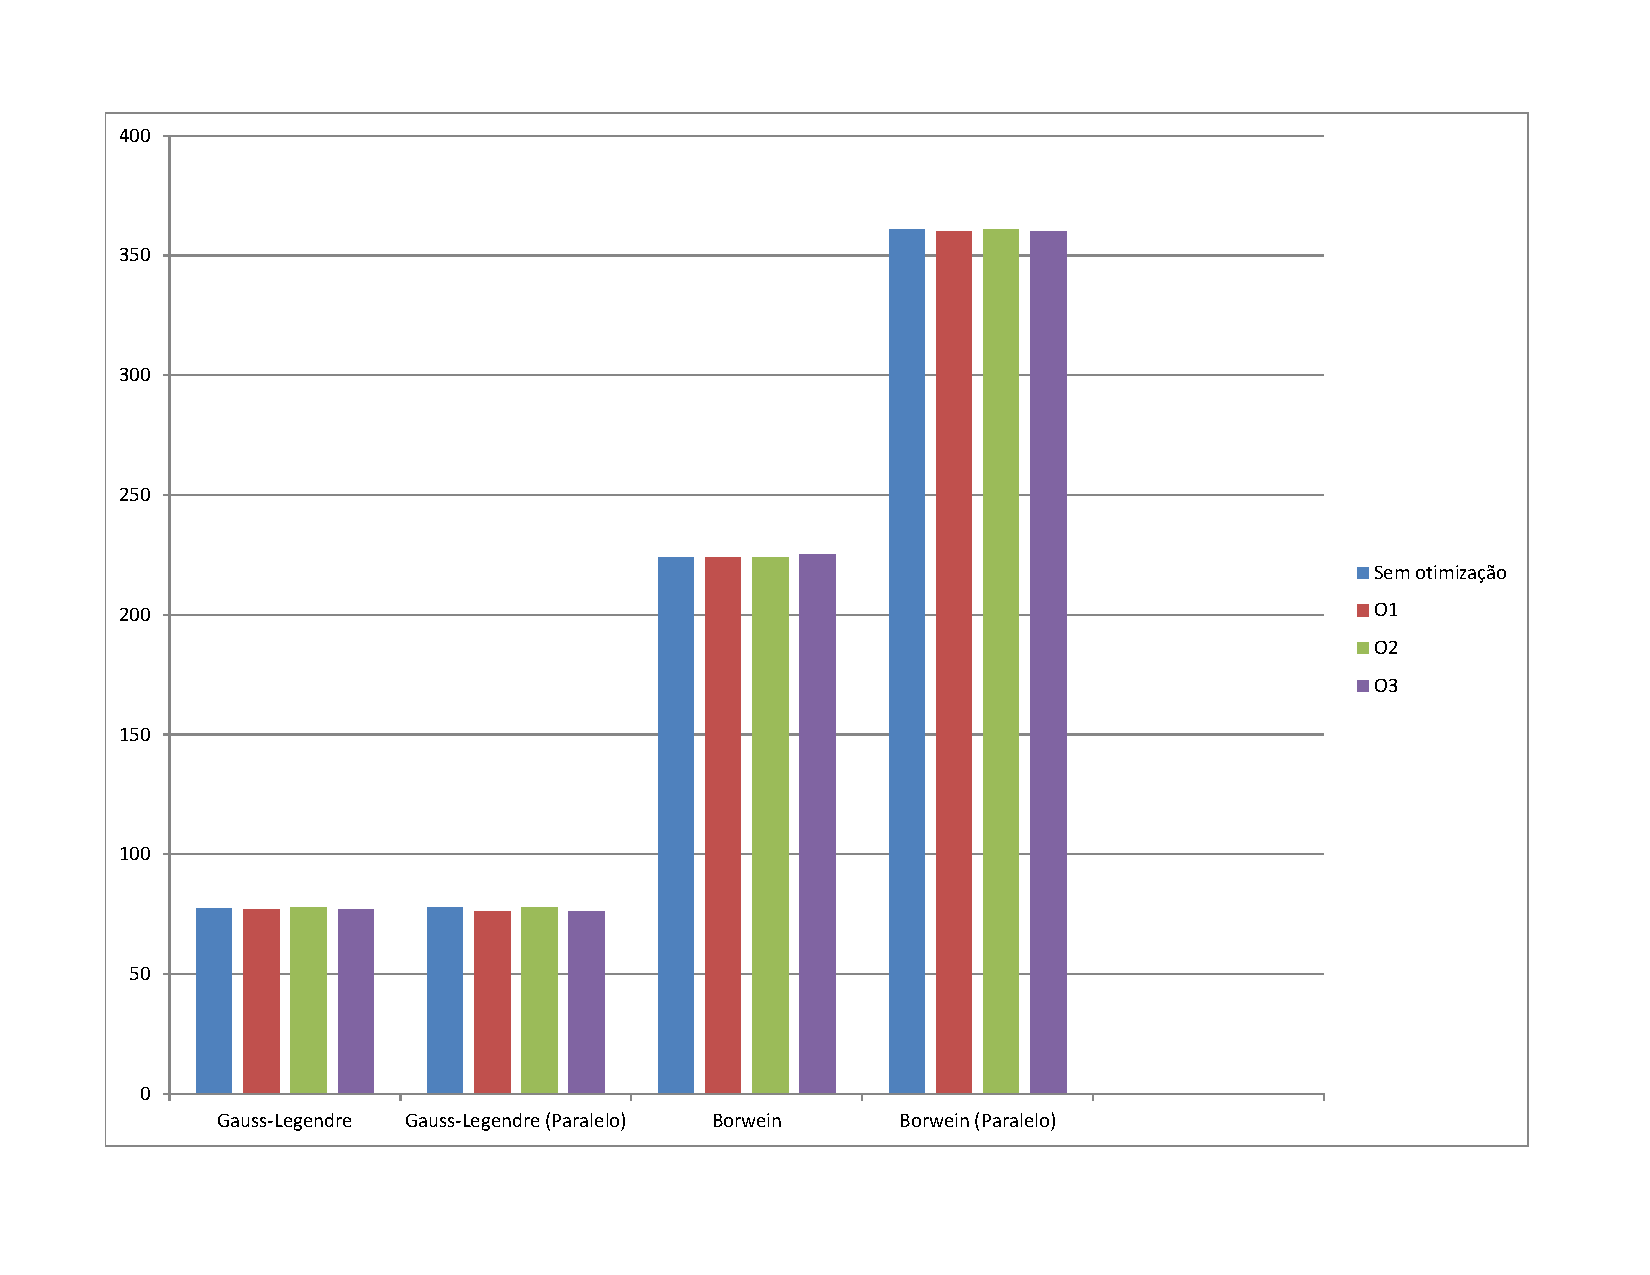
\includegraphics{gauss-borwein}}
	\end{center}
	\caption{Resultados dos algoritmos de Gauss-Legendre e Borwein}
\end{figure}
\begin{figure}[float=h]
	\begin{center}
		\scalebox{0.5}{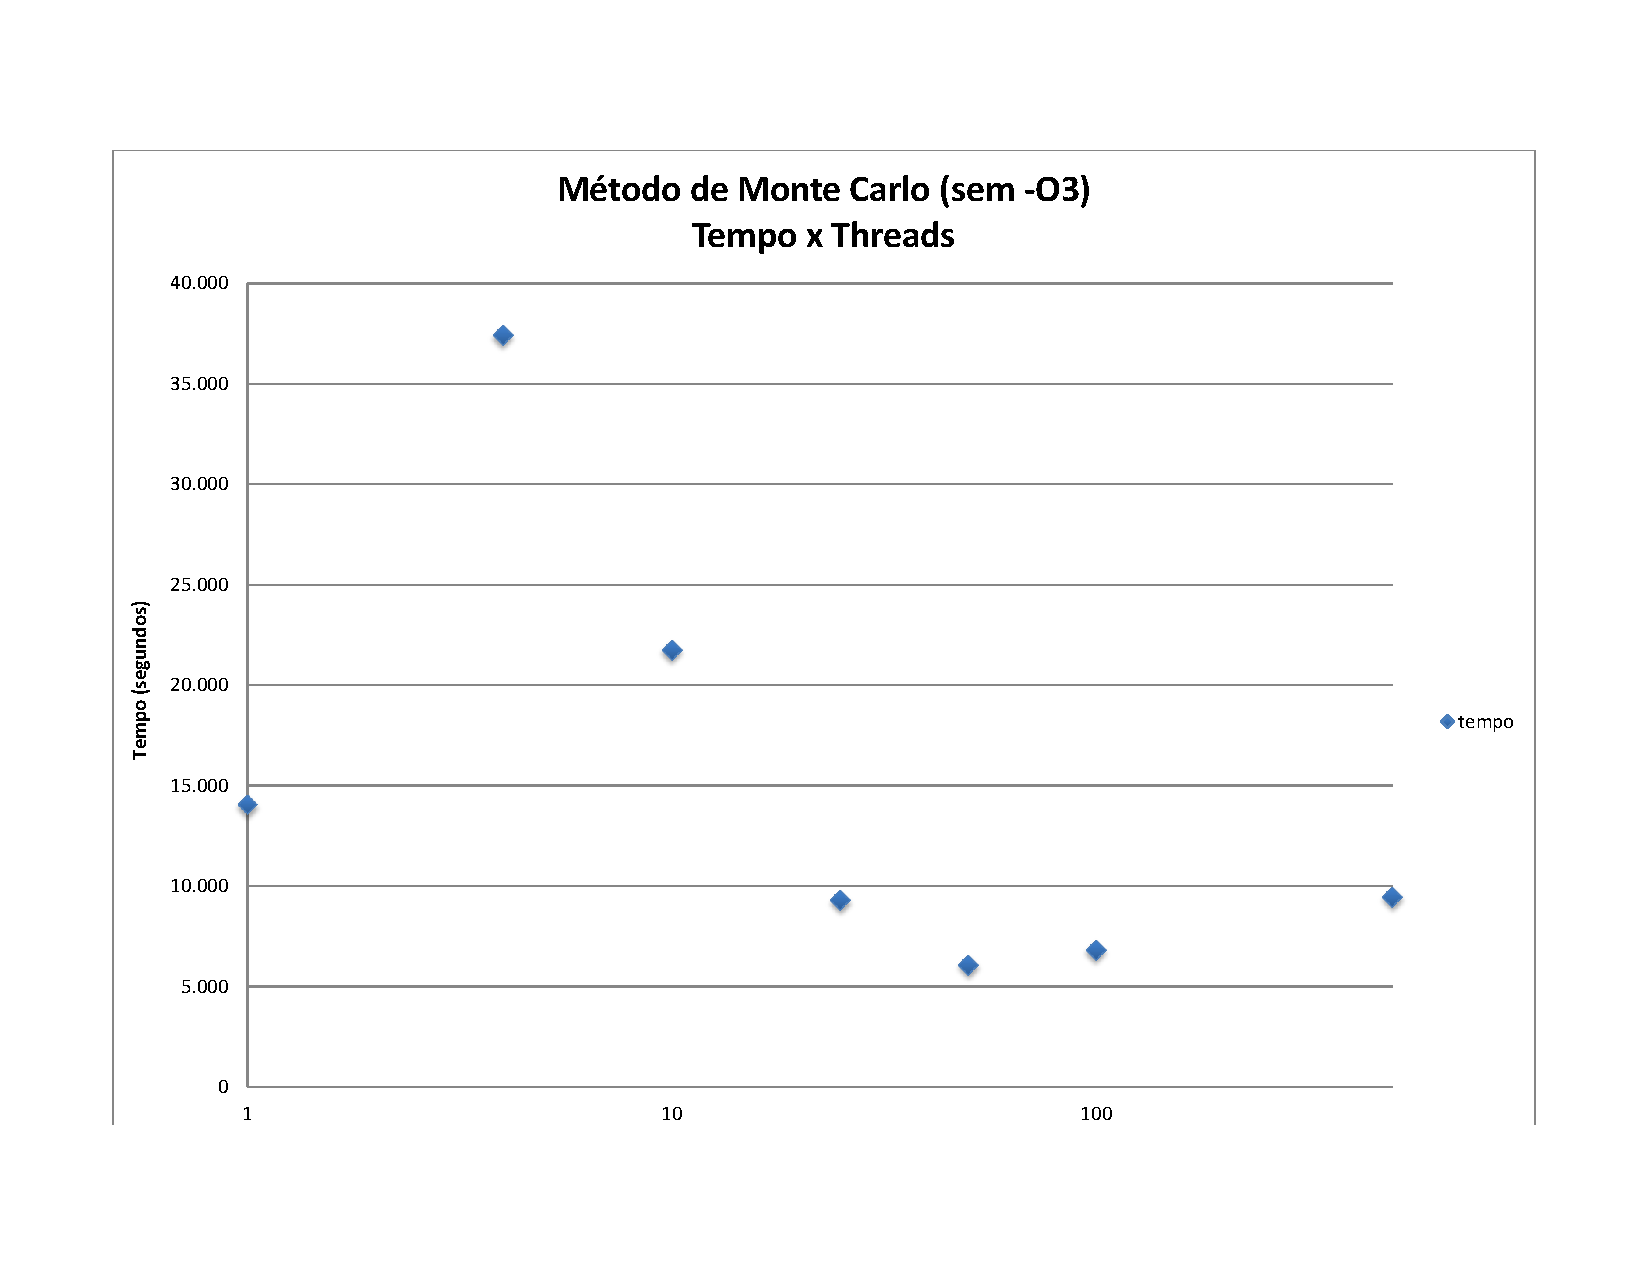
\includegraphics{mc}}
	\end{center}
	\caption{Resultados do algoritmo de Monte Carlo sem otimização}
\end{figure}
\begin{figure}[float=h]
	\begin{center}
		\scalebox{0.5}{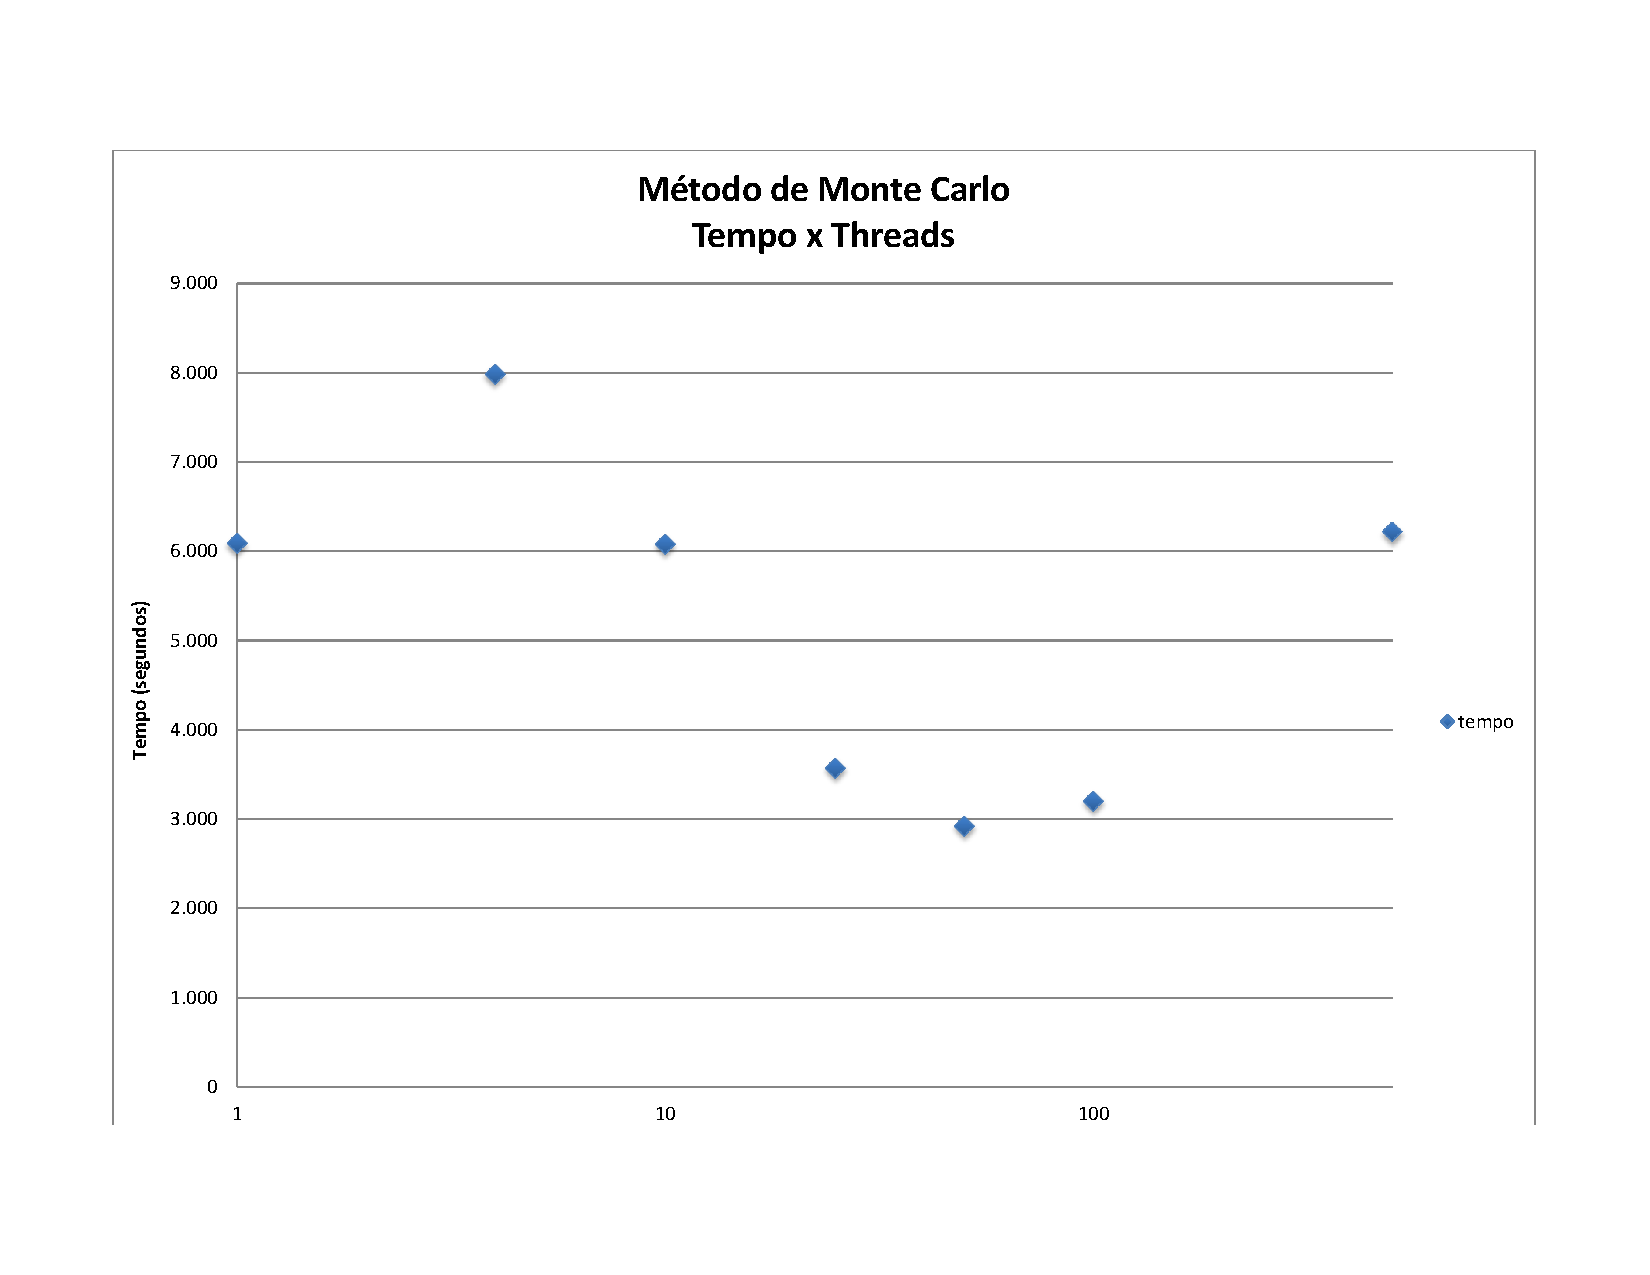
\includegraphics{mcO3}}
	\end{center}
	\caption{Resultados do algoritmo de Monte Carlo com otimização}
\end{figure}

Observando os resultados nas figuras de 1 a 3, para o método de Monte Carlo, é possível concluir que o 
número ideal de threads depende da quantidade de núcleos/unidades de processamento
do computador utilizado. Se este número é pequeno, não será utilizado toda a capacidade 
de processamento, se o número é grande, o overhead do escalonamento do sistema operacional 
para alocar o processamento de cada thread (no caso número de threads >> unidades de processamento) 
será muito grande, deixando lento o método. Para os outros métodos, esse fato também
pode ser considerado. Os algoritmos de Gauss-Legendre e Borwein, como são iterativos,
tiveram apenas um pequeno ganho de tempo. Isto é, cada iteração depende da anterior,
fazendo com que a abordagem paralela não seja muito chamativa. Em especial, no
algoritmo de Borwein, a implementação não é eficiente, já que para calcular \begin{math}a_{k+1}\end{math}, 
é necessário esperar o resultado de \begin{math}y_{k+1}\end{math}. No algoritmo de
Gauss-Legendre, há essa dependência apenas para \begin{math}a_{n+1}\end{math} e \begin{math}t_{n+1}\end{math}. Este pequeno ganho nos
métodos também pode ser duvidável, visto que outros processos no computador 
estavam sendo executados, podendo influenciar no cálculo do tempo de execução. 

\section{README}
Cada algoritmo está implementado em um arquivo único. As implementações do método
serial estão separadas do método paralelo, usando o sufixo \emph{-threaded} no nome do arquivo.
Um arquivo makefile foi criado para facilitar a compilação dos códigos. Para compilá-los,
basta executar \emph{make release}. As bibliotecas GNU MP e pthreads devem estar
instaladas para o sucesso da operação. Os binários serão gerados na mesma pasta.

\section{Referências}
\begin{itemize}
\item http://pubs.opengroup.org/onlinepubs/009695399/functions/rand.html
\item http://www.gnu.org/software/libc/download.html
\item http://cer.freeshell.org/renma/LibraryRandomNumber/
\item http://en.wikipedia.org/wiki/Linear\_congruential\_generator
\item http://mathworld.wolfram.com/MonteCarloMethod.html
\item http://www.chem.unl.edu/zeng/joy/mclab/mcintro.html
\item http://en.wikipedia.org/wiki/Native\_POSIX\_Thread\_Library
\item http://www.icir.org/gregor/tools/pthread-scheduling.html
\item http://en.wikipedia.org/wiki/Gauss-Legendre\_algorithm
\item http://en.wikipedia.org/wiki/Borwein's\_algorithm
\end{itemize}
\end{document}
